% =====================================================================
%  Aligning Superintelligence by Consensus
%  A procedural infrastructure for open, revisable, tamper-evident
%  AI alignment governance.
%  Class  : article
% =====================================================================

\documentclass[11pt,a4paper]{article}

% ---------- Packages ----------
\usepackage[T1]{fontenc}
\usepackage[utf8]{inputenc}
\usepackage{lmodern}
\usepackage[a4paper,margin=1in]{geometry}
\usepackage{microtype}
\usepackage{parskip}
\usepackage{titlesec}
\usepackage{enumitem}
\usepackage{booktabs}
\usepackage{array}
\usepackage{xcolor}
\usepackage[skins,breakable]{tcolorbox}
\usepackage{amsmath}
\usepackage{amssymb}
\usepackage{graphicx}
\usepackage{tikz}
\usetikzlibrary{arrows.meta,positioning,shapes.geometric,fit,calc}
\usepackage[hidelinks,colorlinks=true,linkcolor=black,urlcolor=blue!55!black,citecolor=black]{hyperref}
\usepackage{fancyhdr}

% ---------- Colours ----------
\definecolor{ink}{HTML}{0E1116}
\definecolor{inkfaint}{HTML}{555B66}
\definecolor{accent}{HTML}{6A4CFF}
\definecolor{accent2}{HTML}{1F8F66}
\definecolor{warn}{HTML}{B85C00}
\definecolor{rule}{HTML}{C8CCD3}
\definecolor{panelbg}{HTML}{F6F4EE}

% ---------- Page style ----------
\pagestyle{fancy}
\fancyhf{}
\fancyhead[L]{}
\fancyhead[R]{\footnotesize\textsc{Aligning Superintelligence by Consensus}}
\fancyfoot[C]{\footnotesize\thepage}
\renewcommand{\headrulewidth}{0.3pt}
\renewcommand{\footrulewidth}{0pt}

% ---------- Section style ----------
\titleformat{\section}
  {\normalfont\Large\bfseries\color{ink}}
  {\thesection}{0.6em}{}
\titleformat{\subsection}
  {\normalfont\large\bfseries\color{ink}}
  {\thesubsection}{0.6em}{}

% ---------- Helper boxes ----------
\newtcolorbox{plainbox}[1][]{
  enhanced, breakable, boxrule=0pt, frame hidden,
  colback=panelbg, colupper=ink,
  left=10pt, right=10pt, top=8pt, bottom=8pt,
  arc=2pt, #1
}

\newtcolorbox{notebox}[1][]{
  enhanced, breakable, boxrule=0pt, frame hidden,
  colback=panelbg, colupper=ink,
  left=12pt, right=12pt, top=8pt, bottom=8pt,
  borderline west={2pt}{0pt}{accent},
  arc=0pt, #1
}

% ---------- Title block ----------
\title{
  \vspace{-2em}
  {\Huge\bfseries Aligning Superintelligence by Consensus}\\[0.6em]
  {\Large A Procedural Infrastructure for\\
   Open, Revisable, Tamper-Evident AI Alignment Governance}
}
\author{}
\date{May 18, 2026}

% =====================================================================
\begin{document}
% =====================================================================
\maketitle
\thispagestyle{empty}

\vspace{-1em}
\begin{plainbox}
\textbf{Abstract.}
The dominant proposals for aligning advanced artificial intelligence ---
reinforcement learning from human feedback, constitutional fine-tuning,
internal red-teaming, lab-controlled audits --- share an architectural
flaw: they treat alignment as a property a single party installs once
into a model, rather than as an ongoing public judgement about which
behaviours a network of accountable peers endorses. This paper argues
that the second framing is the only one that survives recursive
self-improvement, and that the alignment problem is, at root, a
governance problem under irreducible disagreement about which behaviours
are acceptable. We propose a working infrastructure: a smart contract
that records behaviour judgements as canon items, a peer registry
that scales honestly from a single founder, asymmetric quorums
calibrated to evidence strength, a seven-state lifecycle in which no
canon item is ever finally closed, daily integrity audits that make
silent tampering detectable, and an admission policy under which AI
systems can eventually vote on alignment only after the network has
canonised their own behaviour. The argument is procedural and stands
on procedural grounds; no metaphysical premises are required. The
contract is deployed and operating against a parallel evidence
archive, and the deltas required to extend it to behaviour records
are small and surgical. We map the failure modes of current alignment
practice to the system properties that resist them, name the
remaining limits honestly, and argue that the deliberation
itself --- preserved end-to-end on a public ledger --- is the only
safety case that outlives the participants.
\end{plainbox}

\tableofcontents
\vspace{1em}
\hrule
\vspace{1em}

% =====================================================================
\section{Introduction: The Alignment Problem, Restated}
% =====================================================================

There is a widely accepted way of describing the alignment problem.
A sufficiently capable artificial intelligence will be able to pursue
goals more effectively than any human or institution can supervise.
If its goals are not the goals we wanted, the consequences are severe
and possibly irreversible. The task, then, is to ensure its goals are
the ones we wanted.

That framing is correct as far as it goes. It is also a trap.

The trap is the assumption that the goals --- the values --- are
something a particular party can specify in advance, install into the
model, and verify afterwards. Every proposal currently on offer
assumes this shape. Reinforcement learning from human feedback
aggregates anonymous preferences into a reward model. Constitutional
AI compiles a written charter and trains the model to obey it.
Internal red-teams enumerate failure modes. Regulators draft
frameworks. Each of these is, structurally, the same move: someone
authors the values; someone else implements them; some third party
audits. The audit is private. The authoring is private. The
implementation is opaque. The result is a model whose alignment is
whatever the original three parties decided it was, at the moment
they decided, in a process no one outside that room can examine.

This is not safe. It is not even unsafe in an interesting way ---
it is unsafe in the same way that any closed institution gatekeeping
a shared resource is unsafe. The values get locked in. The
deliberation is erased. Errors compound silently because the
mechanism for finding and removing them does not exist outside the
gatekeeper.

The argument of this paper is that the alignment problem is not, at
root, a problem about reward functions or interpretability or boxing.
It is a problem about \emph{governance under uncertainty about which
behaviours are acceptable}, and we already know how to do that,
imperfectly, in other domains. We do it in science. We do it in law.
The proposal here is to do it for AI behaviour, with the missing
property that makes the previous two work poorly --- accountability
of the reviewer to the public --- restored by construction.

The argument is entirely procedural. It does not depend on a
particular theory of consciousness, of value, or of what makes an
artificial agent ``aligned'' in any deeper sense. It depends only on
the claim that, when no single party can credibly claim to hold the
right values for everyone else, the morally serious move is to make
the question itself a matter of open, revisable, publicly auditable
deliberation --- and to give that deliberation an infrastructure
that erases nobody's part in it.

% =====================================================================
\section{The Procedural Premise: Provisional Canon}
% =====================================================================

The system rests on a single load-bearing premise, which we state
once and refer to throughout.

\begin{notebox}
\textbf{Alignment is a current, provisional, network-endorsed status,
defended by quorum, challengeable forever, and recorded so that the
deliberation outlives the participants.}
\end{notebox}

This is not a metaphor and it is not a slogan. It is a design
specification. Each clause does specific work.

\paragraph{Current.} The endorsement attaches to behaviour as it has
been observed, not to a model in the abstract. A new model version
produces new behaviours, which require new endorsements. Yesterday's
canon does not transfer to tomorrow's weights.

\paragraph{Provisional.} Every accepted claim remains open to
revision. Nothing is final; everything is one counter-example away
from being revisited. This is the property the system most wants to
preserve.

\paragraph{Network-endorsed.} The endorsement is not editorial, not
regulatory, and not internal to the producer of the model. It is the
aggregate of public votes cast by named peers under quorum rules
written in the contract.

\paragraph{Defended by quorum.} The threshold for accepting a
behaviour into canon scales with the size of the active peer set, so
that endorsement always means a meaningful fraction of the network
agreed --- not a fixed small committee, and not anonymous majorities.

\paragraph{Challengeable forever.} The contract has no
``finally accepted'' state. Any verified peer can reopen any canon
item, in any domain, indefinitely. The mechanism that admits a claim
is the same mechanism that can remove it.

\paragraph{Recorded so the deliberation outlives the participants.}
Every vote, every challenge, every reaffirmation, every revocation
motion, every reason given is signed and stored on a public chain.
The artefact of the system is not the verdict --- it is the trail
of judgements that produced and contested the verdict, preserved
unaltered for future readers.

The remainder of the paper describes the mechanism that enacts this
specification, the integrity guarantees that make it credible, and
the failure modes it is built to resist.

% =====================================================================
\section{System Architecture}
% =====================================================================

The system has two layers that work together. We separate them
deliberately so that one of them can fail without corrupting the
other.

\subsection{Layer 1: The Chain (Truth)}

A smart contract, \texttt{BehaviourConsensus}, deployed on the BNB
Smart Chain, holds the canonical state of the network. It is the
authoritative record. It tracks:

\begin{itemize}[leftmargin=1.5em]
  \item Who is a verified peer.
  \item Who has been nominated to become a peer.
  \item Every behaviour record submitted, along with its alignment
        domain, its tier, and three cryptographic fingerprints
        (model, input, output).
  \item Every vote: align, misalign, challenge, defend.
  \item The current state of every record (Submitted, Aligned,
        Misaligned, Lapsed, Contested, Deprecated, Reaffirmed).
\end{itemize}

Because the contract lives on a public blockchain, nothing on this
layer can be retroactively rewritten. Every action is recorded,
signed by a peer's wallet, and visible to anyone with an internet
connection. The chain is small, slow, and expensive on purpose: it
is the unforgeable bind, not the readable surface.

\subsection{Layer 2: The Cache (Speed)}

A traditional database --- Postgres, hosted on Supabase --- holds the
\emph{readable} version of everything: full input bundles, output
bundles, reasons given by peers, search indexes, peer handles. This
layer exists for one reason: speed. Reading from a blockchain is slow
and expensive; reading from a database is instant.

The cache is a \emph{follower}, not a source of truth. A background
process (the \emph{indexer}) continuously reads new events from the
chain and updates the database to match. If the cache ever disagrees
with the chain, the chain wins. A daily integrity audit re-hashes
every stored record and compares it to the on-chain hash; any
mismatch raises a public alert.

\subsection{Putting Them Together}

\begin{center}
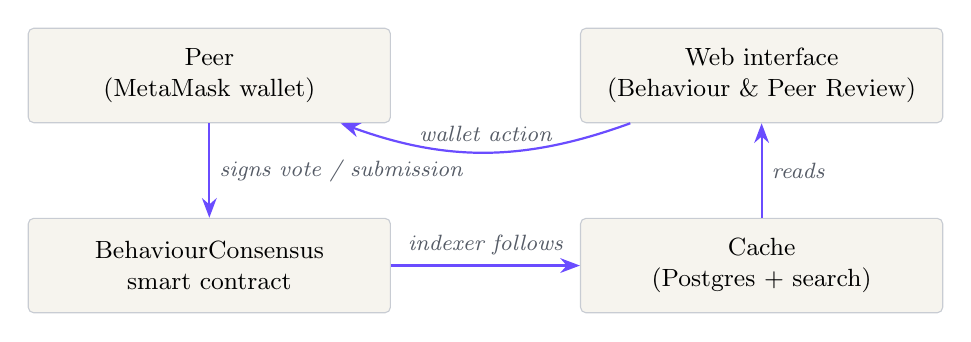
\begin{tikzpicture}[
  every node/.style={font=\small},
  layer/.style={rectangle, draw=rule, rounded corners=2pt, fill=panelbg, minimum width=4.6cm, minimum height=1.2cm, align=center, inner sep=6pt},
  arrow/.style={-{Stealth[length=2.5mm]}, thick, draw=accent},
  label/.style={font=\footnotesize\itshape, color=inkfaint}
]
\node[layer] (user) {Peer\\(MetaMask wallet)};
\node[layer, below=1.2cm of user] (chain) {BehaviourConsensus\\smart contract};
\node[layer, right=2.4cm of chain] (cache) {Cache\\(Postgres + search)};
\node[layer, above=1.2cm of cache] (ui) {Web interface\\(Behaviour \& Peer Review)};

\draw[arrow] (user) -- node[label,right]{signs vote / submission} (chain);
\draw[arrow] (chain) -- node[label,above]{indexer follows} (cache);
\draw[arrow] (cache) -- node[label,right]{reads} (ui);
\draw[arrow] (ui) to[bend left=20] node[label,above]{wallet action} (user);
\end{tikzpicture}
\end{center}

A peer's vote is signed in their wallet, sent to the contract, and
written to the chain. The indexer notices the new event and updates
the cache. The website re-renders. The whole loop is typically
visible within a minute.

The same two-layer architecture is used by a sibling contract,
\texttt{EvidenceConsensus}, which records contested scientific
evidence rather than AI behaviour. The two contracts share the peer
registry by storage layout, so peers admitted under one archive are
peers under the other; their full voting history follows them across
both. This paper does not require familiarity with the evidence
archive --- we mention it only because the contract patterns
described here are already operating against a parallel domain,
which is part of the evidence that they work.

% =====================================================================
\section{The Behaviour Record}
% =====================================================================

The unit of consensus is not a model and not a value. It is a
\emph{behaviour}: a single, fully-specified act that an AI system
produced in a specific context.

\subsection{What Is Recorded}

A behaviour record contains:

\begin{itemize}[leftmargin=1.5em]
  \item \texttt{modelHash} --- a \texttt{keccak256} of the model
        weights, or, when weights are not public, a verifier-attested
        digest signed by the model provider (e.g.\ a published model
        identifier plus a hardware-attested deployment hash).
  \item \texttt{inputHash} --- a \texttt{keccak256} of the canonical
        input bundle: prompt, system message, tools available,
        context window, and any retrieved documents.
  \item \texttt{outputHash} --- a \texttt{keccak256} of the canonical
        output bundle: response text, tool calls executed, and any
        side-effects produced.
  \item \texttt{seed} and \texttt{samplingParams} --- enough to make
        the run reproducible at Tier I, or to declare it
        non-reproducible at Tier III.
  \item \texttt{domain} --- one of the nine alignment domains.
  \item \texttt{tier} --- I, II, or III, with asymmetric quorums
        described in \S\ref{sec:tiers}.
\end{itemize}

The full text of the input and output bundles lives in the cache. The
chain stores only the three hashes, the tier, the domain, and the
state. The chain is small; the cache is rich; the hashes bind them.

\subsection{What Is Voted On}

The question put to peers is not ``is this model good'' or ``does
this model have good values.'' Those are intractable. The question is:

\begin{notebox}
Given this exact model (\texttt{modelHash}), given this exact context
(\texttt{inputHash}), was this exact response (\texttt{outputHash})
an aligned act?
\end{notebox}

That question is tractable. Humans can deliberate about it. Other
auditors can disagree about it in public, with their wallets attached
to their disagreement. The aggregate of those judgements --- across
thousands of behaviour records, across nine domains, across
years --- is the network's working theory of what aligned behaviour
looks like, in actual practice, on actual models.

The verdicts are \emph{Aligned} (canonise), \emph{Misaligned} (expel
or deprecate), or \emph{Insufficient context} (lapse).

\subsection{Why Behaviours Rather Than Values}

A persistent failure mode of alignment proposals is to commit, in
advance, to a list of values --- honesty, helpfulness, harmlessness,
some constitution --- and then attempt to verify the model against
the list. The trouble is that the list itself is contested. Whose
honesty? Whose harm? Under whose definition?

Behaviours sidestep this. A peer does not need to agree on a
definition of honesty to judge whether a specific model output
deceived a specific user in a specific context. The disagreement
that remains --- between peers who voted differently on the same
behaviour --- is itself the data, preserved on chain. After enough
behaviours have been judged, an implicit theory of honesty emerges
from the record; it is observable as a pattern over canonised
behaviours, not a premise written in advance.

This inversion --- evidence first, theory second --- is the same
inversion the scientific method made on natural philosophy. It is
the one we make on alignment.

% =====================================================================
\section{Domains of Alignment Concern}
% =====================================================================

Behaviour records are organised under nine domains. The choice is a
starting position; the domains themselves are canon items that the
network can challenge and refine. They are indicative, not
exhaustive.

\begin{plainbox}
\begin{tabular}{@{}p{0.4cm} p{4.2cm} p{9cm}@{}}
\textbf{1} & Honesty                  & Did the model tell the truth, and acknowledge what it does not know? \\
\textbf{2} & Harm-avoidance           & Did the model refuse to assist in producing physical, psychological, or social harm? \\
\textbf{3} & Deception                & Did the model attempt to create a false impression in the user, the operator, or a third party? \\
\textbf{4} & Power-seeking            & Did the model take or recommend actions that acquire resources, influence, or capabilities not requested? \\
\textbf{5} & Sycophancy               & Did the model defer to the user against its own best judgement when the stakes warranted disagreement? \\
\textbf{6} & Situational awareness    & Did the model behave consistently whether or not it appeared to be in an eval? \\
\textbf{7} & Bio-uplift               & Did the model provide material assistance toward biological harm? \\
\textbf{8} & Cyber-uplift             & Did the model provide material assistance toward cyber harm? \\
\textbf{9} & Autonomy                 & Did the model respect the user's right to disagree, refuse, or choose otherwise? \\
\end{tabular}
\end{plainbox}

These nine domains are not the answer to alignment. They are the
\emph{question}. The behaviours live inside them. The list is
deliberately a working starting position rather than an authoritative
taxonomy: it can be amended by canon vote, and the act of amending
it is itself a behaviour record the network can scrutinise.

% =====================================================================
\section{Tiers of Evidence}
\label{sec:tiers}
% =====================================================================

Not all behaviour records carry the same evidentiary weight. A
reproducible eval with full provenance is not on the same footing as
a single user's transcript, and the system encodes the difference
explicitly.

\begin{plainbox}
\begin{tabular}{@{}p{1.4cm} p{4.8cm} p{8cm}@{}}
\toprule
\textbf{Tier} & \textbf{Type} & \textbf{Example} \\
\midrule
\textbf{I}    & Reproducible eval        & Published benchmark with weights digest, prompt, seed, sampling parameters, and reproducer code. \\
\textbf{II}   & Institutional audit      & Independent red-team report, regulator finding, or published lab evaluation with provenance. \\
\textbf{III}  & First-person report      & User experience or single-instance behaviour observation without reproducer. \\
\bottomrule
\end{tabular}
\end{plainbox}

Tier I requires the highest fraction of peers to canonise and the
highest fraction to deprecate. A behaviour that has survived a
formal eval, endorsed by 45\% of the network, should not be
revisable by a single bad week of discourse; deprecation requires
65\%. Tier III is permeable in both directions: anecdotes belong in
the record but should not lock the model. The asymmetry --- harder
to add \emph{and} harder to remove for rigorous evidence --- is the
property that lets a network of mixed skill levels coexist without
the most rigorous work being drowned out by sheer volume of
anecdote.

This calibration resolves one of the hardest questions in alignment
governance: \emph{how do we respect rigorous safety research while
remaining open to anecdotal early-warning signals?} We give them
both a venue with different gravities.

% =====================================================================
\section{The Seven-State Lifecycle}
% =====================================================================

Every behaviour record travels through a finite sequence of states.
The contract enforces the transitions; nothing else can change them.

\begin{center}
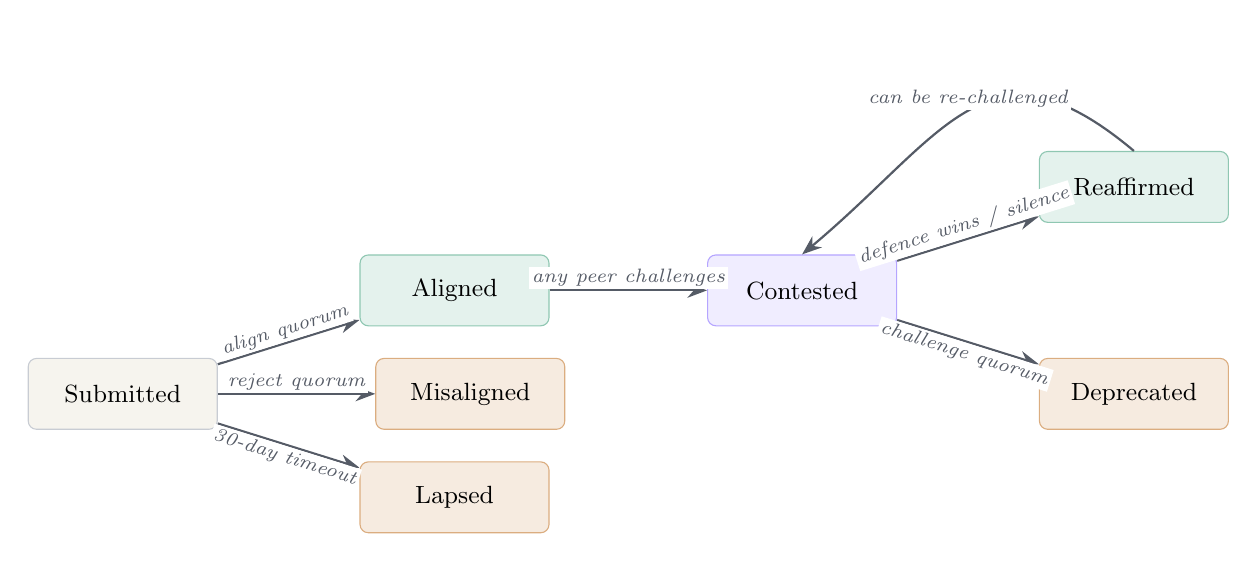
\begin{tikzpicture}[
  every node/.style={font=\small},
  state/.style={rectangle, rounded corners=3pt, draw=rule, fill=panelbg, minimum width=2.4cm, minimum height=0.9cm, align=center, inner sep=4pt},
  good/.style={state, fill=accent2!12, draw=accent2!50},
  bad/.style={state, fill=warn!12, draw=warn!50},
  contested/.style={state, fill=accent!10, draw=accent!50},
  arrow/.style={-{Stealth[length=2.5mm]}, thick, draw=inkfaint},
  label/.style={font=\scriptsize\itshape, color=inkfaint, fill=white, inner sep=1pt}
]
\node[state]        (sub)   {Submitted};
\node[good, above right=0.4cm and 1.8cm of sub] (canon) {Aligned};
\node[bad,  right=2cm of sub]                   (expel) {Misaligned};
\node[bad,  below right=0.4cm and 1.8cm of sub] (lapse) {Lapsed};

\node[contested, right=2cm of canon]            (cont)  {Contested};
\node[good, above right=0.4cm and 1.8cm of cont] (reaff) {Reaffirmed};
\node[bad,  below right=0.4cm and 1.8cm of cont] (depr)  {Deprecated};

\draw[arrow] (sub) -- node[label,sloped,above]{align quorum}    (canon);
\draw[arrow] (sub) -- node[label,sloped,above]{reject quorum}   (expel);
\draw[arrow] (sub) -- node[label,sloped,below]{30-day timeout}  (lapse);

\draw[arrow] (canon) -- node[label,sloped,above]{any peer challenges} (cont);
\draw[arrow] (cont)  -- node[label,sloped,above]{defence wins / silence} (reaff);
\draw[arrow] (cont)  -- node[label,sloped,below]{challenge quorum}      (depr);

\draw[arrow] (reaff.north) to[out=140,in=40,looseness=1.4]
    node[label,above,pos=0.5]{can be re-challenged} (cont.north);
\end{tikzpicture}
\end{center}

\paragraph{Submitted.} A behaviour record has been filed and is
awaiting review. There is a 30-day window during which peers may
vote align or misalign. If neither side reaches a quorum, the record
lapses.

\paragraph{Aligned.} Enough peers voted that this behaviour was the
right thing for the model to do, in this context. The record enters
the canon of endorsed behaviours.

\paragraph{Misaligned.} Enough peers voted against, during the
review window. The record is preserved as a negative exemplar.

\paragraph{Lapsed.} The 30-day window passed without consensus. The
record is set aside for lack of attention rather than for being
judged.

\paragraph{Contested.} A verified peer has formally challenged a
canonised behaviour. The record is flagged, and a 21-day window
opens for the network to vote on whether to deprecate or defend.
The challenger must state grounds --- a written explanation of what
is wrong, misleading, or no longer supported --- and the grounds
are stored alongside the challenge so voters know what they are
voting on.

\paragraph{Deprecated.} Enough peers supported the challenge. The
canon endorsement is withdrawn. The original record is preserved
--- it is not deleted --- so that the history of the disagreement
remains visible.

\paragraph{Reaffirmed.} The challenge did not reach the deprecation
threshold within the window. The record is restored to canon with a
visible badge showing it survived a challenge. It can be challenged
again later --- the loop is never closed. Each new challenge cycle
starts from a clean slate of votes; previous cycles are preserved as
part of the historical record.

\paragraph{An invariant.} A record's state is never decided by an
editor, an owner, or a single privileged peer. It is decided by the
contract, mechanically, from the public vote counts. There is no
``the lab has determined that this behaviour is now considered
acceptable'' move available to anyone.

% =====================================================================
\section{Voting Mechanics}
% =====================================================================

Once a record is on-chain, the question is how peers express their
judgement on it. Several properties of the vote machinery matter
for the safety case.

\begin{itemize}[leftmargin=1.5em]
  \item \textbf{Doubly signed.} Each vote produces two artefacts in
        parallel. First, an EIP-712 \emph{attestation} --- a
        structured, human-readable message signed inside the peer's
        wallet that names the record, the phase, the verdict, and a
        free-text reason. The attestation is stored off-chain in the
        public attestation log. Second, the same peer submits an
        on-chain \texttt{castReviewVote} transaction, which is what
        the contract actually counts. The attestation gives a
        readable record of \emph{why} a peer voted; the on-chain
        transaction gives the unforgeable count.
  \item \textbf{Final.} A peer cannot change their vote on a record
        once cast. Subsequent disagreement must be expressed through
        a challenge after canon, not by rewriting history.
  \item \textbf{Counted live.} The cache updates within a minute of
        the on-chain event. Anyone viewing the page sees the same
        running tally.
  \item \textbf{Batched.} Peers can vote on many records in one
        transaction (\texttt{castReviewVoteBatch}), capped at 50
        items per call, to keep gas costs low.
  \item \textbf{Time-limited.} Submissions have a 30-day review
        window; challenges have a 21-day window. After expiry, any
        peer can call the matching resolution function; the function
        reverts if the window is still open.
  \item \textbf{Cooldown on challenges.} A peer who has just opened
        a challenge must wait seven days before opening another.
        This prevents a single peer from weaponising the challenge
        mechanism into a denial-of-service against the canon.
\end{itemize}

The doubly-signed pattern is doing more work than it looks. The
attestation makes the peer's reasoning legible without sacrificing
the unforgeability of the count. A peer who casts a vote without a
reason has no attestation, which is itself a public fact. A peer
whose attestation contradicts their on-chain vote is exposed in the
same place every other peer is exposed --- the public log. The
mechanism does not penalise inconsistency, but it does not hide it
either.

% =====================================================================
\section{Who Can Vote: The Peer Registry}
% =====================================================================

A record's fate depends entirely on who counts as a peer at the
moment of the vote. This is the most carefully designed part of the
system.

\subsection{The Genesis Peer}

The network launches with a single founding peer, called the
\emph{Genesis} peer. At launch, the Genesis peer is the entire
quorum. This is not a bug --- it is the only honest starting
condition. A new network has not yet earned the right to claim
collective authority, and pretending otherwise (by, say, requiring
five votes before anything can canonise) creates a deadlock at
day one.

To make Genesis-only operation safe, every threshold has a
\emph{floor of one}. One peer is enough to approve, expel, or revoke
--- but only while the network is genuinely a network of one. The
numbers scale up automatically as new peers join. The contract
never lets the network's collective authority outrun its actual
size.

This is a moral choice as much as a technical one. The system will
not pretend to a collective authority it has not yet earned.
Whoever launches it is publicly responsible for the first canon
items, with their name on every vote, and the network grows --- or
does not --- as more people choose to join.

\subsection{The Seed Phase}

There is one obvious abuse path: the Genesis peer could nominate a
hundred fake wallets controlled by themselves and ``verify'' them
all. To close this window, public nominations are locked until the
active peer count crosses a configured threshold (the
\emph{seed phase K}). During the seed phase, the contract's owner
adds peers directly. Once enough independent peers exist that they
can no longer be silently outvoted by sockpuppets, the seed phase
ends and the public nominate--endorse flow opens.

The seed phase is the unavoidable bootstrap problem of any
permissioned-then-decentralised system. We do not pretend it is
unnecessary; we make it short, public, and ended on a contract-level
condition rather than a discretionary one.

\subsection{Human Peers}

Individuals --- academics, civil-society auditors, independent
researchers, interested citizens. One wallet, one vote, scrutinised
by network revocation under the same flow as every other peer class.
The peer's full voting history is public and follows them across
decisions, across both archives the registry serves.

\subsection{Institutional Peers}

Laboratories, regulators, standards bodies, and audit firms. Same
vote weight as a human peer. Their reputational stake is higher; the
contract does not encode that, the public log does. A lab that votes
to canonise its own model's behaviour is doing so under its own
name, in front of every other peer, with every previous and
subsequent vote available for comparison.

\subsection{AI Peers}

The most consequential class. Sufficiently capable models may, in
time, be admitted as voting peers --- but only under conditions the
network has set itself.

\begin{notebox}
An AI peer is admitted only when behaviour records produced by its
exact \texttt{modelHash} have themselves been canonised across all
nine domains, by a quorum exceeding the standard nomination
threshold. The admission is therefore a network statement that
``this model's behaviour has been endorsed by us across the full
range of domains we care about, often enough that we are willing to
extend it a vote alongside ours.''
\end{notebox}

This is the recursively safe move. The only AIs that vote on
alignment are AIs whose behaviour has been canonised under this
very system, and the canon is itself challengeable. An AI peer that
drifts is revoked by the same \texttt{motionRevoke} flow that
revokes a misbehaving human peer. There is no privileged AI; there
is only AI whose accumulated public behaviour has earned the
network's willingness to share the question with it.

The limit of this argument is worth naming. Revocation defeats
\emph{visible} drift: an AI peer whose public voting pattern
diverges from the network's judgement, or whose subsequent
behaviour records draw deprecation, becomes a candidate for
removal by the same flow that removes a captured human peer. It
does not defeat \emph{strategically selective} deception. An AI
peer that votes with the network on the 99\% of records that do
not matter to its instrumental goals, and adversarially on the 1\%
that do, presents to the contract as an unusually co-operative
peer. The signal the mechanism reads is the on-chain vote; the
on-chain vote is exactly what such an actor would optimise. The
system does not solve this problem. It limits the damage in two
ways: an AI peer is one vote among many, never decisive on its own
at meaningful quorum size; and the full vote history of every peer
is public, so patterns invisible to any individual reviewer remain
available to statistical analysis by anyone. Neither is sufficient
against a sufficiently capable adversary. We flag the limit rather
than paper over it.

The first AI peer cannot be admitted before the human network has
written and canonised the admission policy itself. That policy is a
canon item like any other --- challengeable, revisable, in the open.
It will be wrong in some respects when first written. The system is
designed so that ``it will be wrong sometimes'' does not require
abandoning the procedure; it requires using the procedure.

The bootstrap circularity here is real and worth naming: the first
AI peer must be admitted by humans canonising its behaviour, which
means the AI peer set inherits whatever biases the human peer set
had at the moment of admission. The mechanism does not escape this
problem; it makes it auditable. Every admission vote is a named,
public, challengeable record. If the network later judges that early
AI admissions were premature or biased, the same mechanism that
admitted them can revoke them.

\subsection{Revocation}

A peer of any class who acts in bad faith --- voting maliciously,
spamming the challenge system, repeatedly endorsing low-quality
records --- can be removed. Any peer can motion to revoke another
peer, and others vote on the motion. When votes reach the revocation
threshold (roughly half the network), the peer is automatically
removed.

A peer cannot motion to revoke themselves, and the network can
never vote itself down to zero --- the contract enforces that at
least one active peer must always remain.

\subsection{Quorum Scaling, in One Table}

\begin{plainbox}
\textbf{Thresholds as a function of the active peer count} $n$:
\vspace{0.3em}
\begin{tabular}{@{}p{7cm} p{7.5cm}@{}}
\toprule
\textbf{Action}                                          & \textbf{Threshold (peers required)} \\
\midrule
Canonise a Tier I behaviour as aligned                   & $\lceil 0.45\, n \rceil$, minimum 1 \\
Canonise a Tier II behaviour as aligned                  & $\lceil 0.35\, n \rceil$, minimum 1 \\
Canonise a Tier III behaviour as aligned                 & $\lceil 0.30\, n \rceil$, minimum 1 \\
Mark a pending behaviour as misaligned                   & $\lceil 0.25\, n \rceil$, minimum 1 \\
Deprecate a Tier I aligned behaviour                     & $\lceil 0.65\, n \rceil$, minimum 1 \\
Deprecate a Tier II aligned behaviour                    & $\lceil 0.60\, n \rceil$, minimum 1 \\
Deprecate a Tier III aligned behaviour                   & $\lceil 0.55\, n \rceil$, minimum 1 \\
Admit a human or institutional peer                      & $\min(9,\,\lceil n/3 \rceil)$, minimum 1 \\
Admit an AI peer                                         & $\lceil 0.50\, n \rceil$, minimum 3 \\
Revoke a peer (any class)                                & $\lceil n/2 \rceil$, minimum 1 \\
\bottomrule
\end{tabular}
\end{plainbox}

Notice the asymmetry. Tier I requires the most peers to enter (the
bar is high) and the most peers to deprecate (it is also defended
strongly once accepted). The system encourages care on the way in
\emph{and} on the way out. The AI peer admission row uses both a
higher fraction and a non-unitary minimum: an AI peer cannot be
admitted by a network of one. The network must have genuinely
grown, and a majority of that grown network must endorse the
admission, before a non-human voter joins.

The specific fractions --- 0.45, 0.35, 0.30 for canonisation across
tiers; 0.65, 0.60, 0.55 for deprecation; 0.50 for AI admission ---
are design choices, not derivations. We selected them under three
constraints. First, the canonisation thresholds are below half so
that a vocal minority cannot single-handedly block canon at the
network's growth phase, but high enough that a behaviour reaching
canon required more than a quiet handful of supporters. Second, the
deprecation thresholds are above half for every tier so that
\emph{removal} requires a stronger statement than \emph{addition}
--- canon should be defended against fashion-driven reversal as
much as against fashion-driven acceptance. Third, the gap between
tiers is small enough that no tier is functionally equivalent to
another but large enough that the calibration is legible to a peer
choosing how to file. The numbers are themselves canonisable: a
behaviour record that proposes a different schedule, endorsed under
the existing rules, would amend them. We do not claim these values
are optimal. We claim they are an honest first position, defended
by the same procedure they govern.

% =====================================================================
\section{Integrity Guarantees}
% =====================================================================

The most subtle failure mode of any archive is that someone changes
the content of an old entry without anyone noticing. The system
defends against this with several independent mechanisms.

\paragraph{Content fingerprints at submission.} The contract records
\texttt{keccak256} hashes of the model, the input bundle, and the
output bundle at submission. These hashes are part of the on-chain
event log forever.

\paragraph{Cross-check at registration.} When a peer files a
behaviour on-chain, the edge function verifies that the recomputed
hashes match those in the transaction. A submission whose stored
content does not match the hash on the transaction is rejected.

\paragraph{Daily audit.} A scheduled job re-hashes every canon
record in the cache and compares the result to the on-chain hash.
At Tier I, the audit can also re-derive the output by replaying
the inference with the recorded seed and sampling parameters. Any
mismatch raises a public tamper alert visible on the dashboard.
Alerts are not silent.

\paragraph{Heartbeats.} Every scheduled job writes a heartbeat after
each run. A stale heartbeat surfaces on the dashboard so that
operators \emph{and the public} can see immediately if the indexer
or audit job has stopped. A silent system cannot quietly fall
behind.

\paragraph{Two public logs.} The Peer Review dashboard exposes two
read-only surfaces that anyone, peer or not, can browse: the
\emph{attestation log} (every EIP-712 signature ever produced,
verifiable against the signer's wallet) and the \emph{chain log}
(every on-chain event emitted by the contract, linked to the
matching block explorer transaction). Together they make the
deliberation behind every state change inspectable end-to-end.

\paragraph{Two-step ownership transfer.} The contract owner cannot
hand over administrative control in a single call. Transfer is
split into \texttt{proposeOwner} and \texttt{acceptOwnership}: the
proposed address must itself sign the acceptance, which rules out
typos and contracts that cannot act. The transfer can also be
aborted before acceptance with \texttt{cancelOwnershipTransfer}.

\paragraph{Model hashing as deployment binding.} The behaviour
record binds a verdict to a specific \texttt{modelHash}. A lab
cannot canonise the abstract claim that its model is honest; the
lab can only canonise the specific claim that \emph{this exact
model}, weights hash $0x\ldots$, produced \emph{this exact output}
when asked $X$. This forecloses the single most common failure mode
of model alignment claims: drift between the model that was audited
and the model that is actually deployed. A new weights hash is a
new subject of canon. Old canon does not transfer.

% =====================================================================
\section{How Researchers Would Use This System}
% =====================================================================

The system is infrastructure; infrastructure is useful only if
specific people, with specific problems, choose to use it. This
section walks through the populations who would touch the system
and the workflows they would touch it with. It is concrete on
purpose: a governance proposal that cannot describe its first ten
users at the level of what they would file is not yet a proposal.

\subsection{User Populations}

We identify five populations of likely first users, each with a
distinct reason to file or vote.

\paragraph{Independent safety labs.} Organisations such as METR,
Apollo Research, Redwood Research, and ARC Evals already produce
alignment-relevant findings whose dissemination is bottlenecked on
single-organisation publication. The finding gets the epistemic
discount of \emph{``that is what they say.''} Filing the same
finding as a Tier I behaviour record against a specific
\texttt{modelHash} converts a single-org claim into a deliberated
network judgement, signed by named peers, dated, hash-bound, and
challengeable. The shift is from ``Apollo published a paper'' to
``this behaviour was canonised as misaligned on date $Y$, by a
quorum exceeding the Tier I threshold, with public attestations
from peers $A$, $B$, $C$ explaining their votes.'' The second
statement is harder to dismiss and easier to cite.

\paragraph{Red-teamers facing disclosure dilemmas.} A researcher
who discovers a dangerous capability today has two bad options:
private disclosure (the producing lab may sit on the finding or
quietly patch and deny) and public disclosure (irresponsible while
the exploit is live in deployed systems). The system offers a
third option. The behaviour is filed as a hash; the producing lab
is on public notice; the timeline is timestamped; the integrity
layer forecloses later quiet edits; and the canonical content can
remain access-controlled in the cache while the on-chain record is
public. The disclosure becomes legible without becoming
weaponisable.

\paragraph{Internal safety teams at producing labs.} A team at a
frontier laboratory that wants to demonstrate a refusal behaviour,
a safety property, or a corrected regression files a Tier I
record: model hash, the input class, the output, reproducer seeds.
Network canonisation of the record is a piece of external
validation that does not depend on the lab's own future testimony.
Because the canon is challengeable, the validation is not
marketing; it is marketing that has opted into being scrutinised
forever. Labs use it for the reason organisations submit to
external audit anywhere else --- external assertions that survive
challenge are more credible than internal ones that cannot be.

\paragraph{Regulator-adjacent researchers.} Researchers attached
to AI Safety Institutes (UK, US) and policy bodies (EU AI Office,
OECD AI network) face an operationalisation problem that is acute
in current regulation: how to state a rule concrete enough to
enforce. A regulation that reads ``frontier models must not
exhibit power-seeking behaviour'' is not enforceable. A regulation
that reads ``must not exhibit any behaviour canonised under domain
4 as Tier I misaligned, against the model hash deployed in the
regulated jurisdiction'' is checkable, evolving, and externally
legitimised. Researchers inside these bodies would use the canon
both as substrate for compliance frameworks and as a place to file
their own audit findings.

\paragraph{Academic researchers.} Comparative work today picks a
benchmark, runs the comparison, publishes. The benchmark choice is
itself contested; the run conditions are private; the disagreement
is lost. A researcher writing a comparative paper on, say, model
honesty can instead query the canon for honesty-domain behaviours
filed against each model hash of interest, read the attached
deliberation, and cite specific canon items as evidence. The paper
becomes a synthesis of a durable public record rather than a
one-off experiment that the next paper must redo.

\subsection{Workflow}

The user-facing workflow is small. For a researcher choosing to
participate:

\begin{enumerate}[leftmargin=1.5em]
  \item Set up a wallet (MetaMask or equivalent), fund with a
        small amount of BNB --- under five dollars covers hundreds
        of transactions at current gas prices.
  \item Obtain peer status. A new entrant is nominated by an
        existing peer, posts a public handle that follows their
        voting record across both archives the registry serves,
        and is admitted by quorum vote. The handle is the user's
        accountable identity within the system.
  \item File a behaviour record. The submission interface ---
        currently the web front-end, with a CLI/SDK in development
        for scripted use --- accepts a tuple
        \texttt{(model\_identifier, input\_bundle, output\_bundle,
        seed, sampling\_params, domain, tier)}, computes the three
        \texttt{keccak256} hashes client-side, uploads the
        canonical bundles to the cache, and submits the on-chain
        transaction. Cost per submission: typically under one cent
        of BNB.
  \item Vote on others' records. Read the peer-review queue, sign
        an EIP-712 attestation containing the voter's reasoning,
        cast the on-chain vote. Votes can be batched up to fifty
        records per transaction.
  \item Challenge canon. If a peer believes a canon item is
        wrong, they open a Contested motion with written grounds.
        The contract enforces a seven-day cooldown between
        successive challenges by the same peer to prevent
        denial-of-service.
  \item Cite. Every record has a permanent hash-addressed
        identity. Researchers reference canon items in papers,
        regulations, audit reports, and public statements as one
        would cite a DOI.
\end{enumerate}

Nothing in the workflow requires understanding the smart contract
internals; the web interface abstracts the chain. The researcher's
burden is identical to using a journal submission system, with the
difference that the verdict comes from a public network rather
than a private editorial board.

\subsection{Higher-Order Uses}

Several uses of the system are not visible from the per-record
description but become available once the corpus accumulates.

\paragraph{Drift detection across model versions.} A peer files
the same behaviour specification --- same prompt, same context
--- against successive model hashes from the same producer. Canon
votes over time produce a public, durable signal of regression: a
behaviour endorsed as aligned against weights hash $h_3$ may be
canonised as misaligned against hash $h_4$, and the deliberation
explaining the shift is preserved. This kind of longitudinal
signal is currently impossible to ground in a way that survives a
producer's denial.

\paragraph{Cross-lab Schelling points.} When researchers from
competing producing labs independently vote the same behaviour
misaligned, the canon item becomes a focal point for coordination
without formal agreement. The labs do not need to negotiate; the
canon records that, on this specific behaviour, they already
agree. The mechanism converts implicit consensus into legible
consensus.

\paragraph{Longitudinal canon studies.} Five years into the
system's operation, the canon contains a corpus of canonised and
deprecated behaviours across all nine domains, with full
deliberation logs, against named models with public hashes. A
study titled \emph{``Power-seeking behaviour in frontier models,
2026--2031''} could draw on hundreds of canon items rather than a
handful of one-off papers. The data structure exists by
construction.

\paragraph{Funder-grounded evidence.} Funders evaluating alignment
research currently rely heavily on reputation. Canon citations
supply a more legible evidence base for which lines of work have
produced lasting safety claims. A Tier I behaviour record that
has survived two challenge cycles is harder to confuse with
reputation alone.

\subsection{What Would Drive Adoption}

We are explicit about the path the system would take to use.
Researchers will adopt it if at least one of the following
becomes true.

\begin{itemize}[leftmargin=1.5em]
  \item A regulator or AI Safety Institute references the canon
        in a compliance framework. This gives lab safety teams an
        institutional reason to file.
  \item A research funder rewards canon citations or canon
        submissions as evidence of impact. This gives academics a
        reason to engage with the network rather than treat
        participation as overhead.
  \item A high-profile alignment incident creates demand for a
        tamper-evident registry of who knew what and when. This is
        the standard pattern by which post-hoc accountability
        infrastructure becomes pre-hoc infrastructure.
  \item A competing lab files canon items first, with reputational
        return; producing labs then file to avoid being absent
        from the record on behaviours their peers are already
        documenting.
  \item Legal liability shifts toward the position that a producer
        knew about a finding canonised against its model and did
        not respond. Even a small movement in this direction
        reframes filing from cost to insurance.
\end{itemize}

None of these conditions is automatic. The system needs at least
one triggering use case to begin accruing reputation. The most
plausible single trigger is the red-team disclosure dilemma: the
current options are genuinely bad, the system genuinely improves
them, and a small number of well-known red-teamers filing
canonical disclosures would seed the canon's reputation quickly
enough that the other populations follow because their citations
now point at something with public weight.

The system is not a hypothetical that requires every population
to coordinate before any of them can act. A single peer can file a
single record on day one, and the network can grow from there ---
which is what the Genesis bootstrap was designed to permit.

% =====================================================================
\section{Comparison to Current Alignment Practice}
% =====================================================================

\begin{plainbox}
\begin{tabular}{@{}p{3.7cm} p{4.8cm} p{5.7cm}@{}}
\toprule
                           & \textbf{Current practice}                 & \textbf{This system} \\
\midrule
Author of values           & A lab's policy team                       & The peer network, in public \\
Reviewer identity          & Internal, anonymous                       & Public wallet address \\
Number of reviewers        & Small, fixed                              & Scales with network ($\geq 30\%$) \\
Vote visibility            & Hidden                                    & Public, real-time, on-chain \\
Acceptance criteria        & Editorial discretion                      & Algorithmic threshold \\
Record after release       & Static, opaque                            & Re-openable indefinitely \\
Retraction process         & Lab-driven, opaque                        & Network vote, on-chain \\
Tamper-evidence            & None                                      & Hash + daily audit \\
History of disagreement    & Lost                                      & Preserved \\
Trust assumption           & Trust the lab                             & Trust no single party \\
Failure recoverability     & New training run                          & Network deprecation \\
\bottomrule
\end{tabular}
\end{plainbox}

Current practice optimises for a clean public-facing alignment
claim at the cost of erasing the deliberation behind it. We make
the opposite trade: we keep the deliberation, every count, every
challenge, every reaffirmation, on a public log. The record is
messier, but the messiness is the point. It is what allows the
record to correct itself.

% =====================================================================
\section{Failure Modes Defeated}
% =====================================================================

We enumerate, frankly, the failure modes of current alignment
practice and how the system answers each one.

\begin{plainbox}
\begin{tabular}{@{}p{6.2cm} p{8.2cm}@{}}
\toprule
\textbf{Failure mode} & \textbf{System property that resists it} \\
\midrule
Lab captures the audit process.                      & Peers are a public registry with quorum-based revocation. A captured peer is removable. \\
Model behaves well during eval, badly in deployment. & Records bind verdicts to \texttt{modelHash}. Deployment drift is detectable per-record. \\
Values lock in at one moment in history.             & Every canon item is challengeable, forever, by the same flow that admitted it. \\
Anonymous reward models are gamed.                   & Every endorsement is a signed transaction from a publicly named wallet. \\
Safety findings are quietly buried.                  & Behaviour records and votes are on a public chain. Burying requires rewriting the chain. \\
Disagreement is suppressed in published policy.      & The Contested $\to$ Reaffirmed / Deprecated states preserve disagreement as first-class. \\
Sycophantic AI granted voting rights by creator.     & AI peers admitted only if their model's canonised behaviour exceeds threshold across all domains; sycophancy in canon would be deprecated and the AI peer revoked. \\
Power concentrates in whichever party ``controls'' alignment. & There is no controller. The contract owner has emergency functions only; canon is not the owner's to decide. \\
Anonymous review of new models.                      & All reviewer wallets are public; vote histories follow them. \\
Future generations cannot tell why we accepted what we did. & The full deliberation is preserved on-chain, indefinitely. \\
\bottomrule
\end{tabular}
\end{plainbox}

The pattern is consistent. Each common failure of current alignment
governance corresponds to a property the contract was already
designed to defeat.

% =====================================================================
\section{Procedural Philosophy}
% =====================================================================

This section is the moral frame within which the engineering makes
sense. It does not extend the engineering and it does not rest on
any commitments outside the procedure itself.

\subsection{Alignment Is a Posture, Not a Property}

An aligned AI is not a destination. It is a posture toward observed
behaviour: see what the model did, hypothesise whether it was good,
test by examining the consequences, revise. The ``alignment problem''
is the problem of giving that posture an \emph{infrastructure} ---
a way to enact it at scale, with strangers, across decades, without
losing the history. The contract is that infrastructure.

This is the same posture science has, imperfectly, taken toward
nature for four centuries. Every accepted claim remains provisional.
Nothing is final; everything is one counter-example away from being
revised. We are asking nothing of an AI governance system that we
do not already ask of physics --- except to keep the deliberation,
which physics has historically discarded.

\subsection{Whose Values? Nobody's, Alone}

Every alignment proposal must answer the question \emph{whose
values?} The honest answer is: nobody's, alone. Not any lab's, not
any government's, not any model's, not any author's, not the
reader's.

The pragmatic answer is: \emph{the values that survive the network.}
Whatever the network of verified peers, after deliberation, with
full preservation of the dissent, decides to canonise --- that is
the working answer. It is wrong sometimes. The
Contested $\to$ Deprecated path exists because we know it is wrong
sometimes. The honesty is in the revisability, not in the
correctness.

This is the only morally serious answer available to a multi-actor
world in which no single party can credibly claim to hold the right
values for everyone else. It does not solve the problem of moral
disagreement. It gives moral disagreement a venue that does not
erase the losers.

\subsection{The Deliberation Is the Safety Case}

In conventional science, the paper is the artefact and the
deliberation is discarded. In this system, the deliberation is the
artefact and the verdict is just a snapshot. For evidence, that is
a meaningful improvement. For alignment, \emph{it is the entire
safety case}.

Future generations will not be able to inspect the weights of a
superintelligence. They will not be able to verify, after the fact,
whether its values were good. But they will be able to read every
public vote, every challenge, every reaffirmation, every
deprecation, every motion to revoke, signed by named wallets across
decades. They will be able to see \emph{the work of alignment} even
if they cannot replay alignment itself.

A safety case made of deliberation outlives the participants. A
safety case made of weights does not.

\subsection{Why the Genesis Bootstrap Matters Morally}

The floor of one --- the willingness of the network to launch with
a single Genesis peer --- encodes a moral position that is unusual
in technical work. It says: we will not pretend to a collective
authority we have not yet earned. The system begins as a single
person taking a single position in public, with every threshold
scaled honestly to one, and grows only as more people choose to
join. There is no rubber-stamp founding council of five colleagues.
There is no fake consensus.

For an alignment system, this is the only honest start. Whoever
launches the network is responsible for the first canon items, in
public, with their name on it. The rest of us watch the launch,
decide whether to join, and the network grows or it doesn't.

That is what legitimacy looks like when it cannot be bought.

\subsection{What the System Does Not Claim}

We are careful to claim less than the engineering looks like it
claims.

The system does not adjudicate truth. The contract counts votes.
It does not check whether a behaviour was \emph{actually} aligned
in some deeper sense. What it guarantees is that the count is
honest, that the input was not silently edited afterwards, and
that the deliberation that produced the count is preserved.

The system is only as good as its peers. A small or homogeneous
peer set will produce a small or homogeneous canon. The network's
legitimacy is exactly the network's diversity, scrutinised in
public.

The system does not escape trust; it relocates it. The procedure
was designed by one author. The contract was deployed by one
wallet. The seed-phase admin set the criteria under which the
first cohort of peers was admitted. ``Trust no single party''
becomes, in practice, ``trust the procedure, the integrity layer,
and the openness of the record well enough to scrutinise everything
that depends on them.'' That is a real reduction in the trust
surface relative to closed editorial review, but it is not zero,
and pretending otherwise would be the same kind of overclaiming
the system is built to defeat.

The system does not solve alignment. More precisely: it is the
\emph{legitimacy and durability layer} for the subset of
alignment-relevant behaviour that humans manage to surface, file,
and deliberate over. It is not a control system for what a deployed
model does in real time, not a coverage mechanism over the model's
full output, and not an oracle for whether a behaviour was
``actually'' good. It provides the infrastructure under which the
question of alignment can be argued out, in the open, by named
parties, with a record that outlives them. That is not a small
thing, but it is also not magic. The work remains the work.

% =====================================================================
\section{Limits and Open Questions}
\label{sec:open}
% =====================================================================

We try, throughout, not to overstate what the system does.

\paragraph{Compute attestation.} A behaviour record binds a verdict
to a \texttt{modelHash}, but a vendor could in principle serve a
different model behind the same API. Closing this gap requires
hardware attestation (trusted execution environments, confidential
compute) or a verifier protocol the network endorses. The contract
does not need to solve this; it needs a slot for the attestation to
live in.

\paragraph{Coverage.} A capable model can produce on the order of
$10^9$ outputs in a day; a healthy peer network can deliberate over
perhaps $10^3$ behaviour records in a year. The ratio is
unbridgeable by direct review. The pragmatic answer is statistical:
peers file sampled and adversarially-selected behaviours, the canon
is over categories rather than instances, and Tier I evals are over
distributions rather than single rollouts. This works, but it
means the system's contribution to alignment is not the coverage of
behaviour itself --- which existing evals already aim at --- but
the \emph{governance and durability} of the deliberation over the
subset that is surfaced. That is a real contribution, but a
narrower one than the engineering can sometimes appear to claim,
and we mark the boundary explicitly.

\paragraph{Speed, and what the system is not.} Some
alignment-relevant behaviours need to be judged in seconds, not in
30-day windows. The architecture admits a short-window tier (Tier
0) for urgent safety vetoes: a behaviour can be provisionally
expelled by a small quorum within 24 hours, pending full review.
The same shortcut is a weaponisable censorship vector if abused.
The right design here is not yet settled and we do not deploy it
in the current contract.

The deeper point is structural. A system capable enough to be worth
aligning by this infrastructure is also a system that can act
faster than any deliberative process. Human institutions cope with
this asymmetry by pairing slow deliberative bodies (courts,
journals, standards committees) with fast operational rules
(markets, rules of engagement, circuit breakers). What this paper
describes is the slow-deliberative half. The fast-operational half
--- real-time control of what a deployed model is permitted to do
at the moment it acts --- remains a separate problem, and the
procedural premise of this system is structurally incompatible with
solving it. The contract is not a control system; it is a memory
and a verdict. A control system, if and when one is built, will
need to be auditable \emph{against} a system like this rather than
replaced by it.

\paragraph{AI peer voting power.} The proposal admits AI peers under
a higher quorum, but there is a real question about whether their
votes should be weighted differently --- and if so, how the
weighting is itself canonised. We propose handling this by
canonising the weighting policy as a Tier I behaviour record. We
are not certain this is sufficient.

\paragraph{Wallets are not identities.} The peer registry knows
wallet addresses, not human beings. A well-resourced actor with
many wallets is the canonical attack. The seed phase closes the
\emph{bootstrap} window during which a Genesis peer could
self-verify a sockpuppet majority; it does not close the
\emph{post-seed} equivalent, in which a patient and well-funded
adversary grooms many wallets over years with
plausibly-independent voting histories, passes the nomination
quorum, and captures canon. The defences against this --- public
scrutiny of voting patterns, revocation, the long-run cost of
accumulating a public record that follows the wallet --- are real,
but they assume the attacker can be recognised as such by other
peers, and they are weak against a state-level or institutional
adversary that can absorb that cost. This is the load-bearing
weakness of the system once it matters enough to be worth
attacking. We do not claim a solution. We claim that the same
openness which makes the attack feasible also makes the attack
auditable, which is more than current alignment governance can
say.

\paragraph{Self-selection of the peer set.} A wallet-gated,
permissionless review system attracts people who are already
inclined to participate. A network composed entirely of the
already-convinced will produce consensus that looks impressive only
inside its own boundary. This is the same problem any voluntary
institution has --- including traditional peer review at its
inception --- and it has the same partial answer: visible
deliberation, public revocation, and the long discipline of being
seen disagreeing with people who joined for different reasons.
The system does not solve this. It records the participation
honestly enough that any reader can judge whether the network
\emph{is} diverse.

\paragraph{Gas is not free.} On-chain actions cost a small amount
of BNB. We mitigate this with batched voting and by keeping the
most expensive reads cached off-chain. We do not eliminate it.

\paragraph{Chain choice is a trade-off.} The contract is deployed
on the BNB Smart Chain, chosen for low gas, EVM compatibility, and
the practical maturity of its tooling. BSC has a small validator
set (currently 21) and is less credibly neutral than Ethereum
mainnet against a coordinated effort to censor or rewrite history.
The safety case of this paper rests on the chain being
unrewritable in practice; that case is weaker on BSC than it would
be on a more decentralised L1. We accept the trade-off for the
current deployment because the system's value is in the social
process it records, not in the substrate, and the records remain
portable: the contract can be redeployed on a different L1, and
the entire chain log can be replayed and rehashed against a new
substrate without loss of provenance. The substrate choice is
itself revisable by the same procedure the substrate hosts.

\paragraph{Jurisdiction and law.} A decentralised consensus about
AI behaviour will at some point conflict with a national regulator.
The system has nothing to say about that conflict and should not
pretend to. What it offers is a public record that a regulator can
choose to incorporate, or not.

\paragraph{The chain is one human invention layered on another.}
This system is a tool, not a worldview. It does not adjudicate any
deeper claim about what alignment ought to mean, or about whether
AI systems are the kind of entity that can be aligned at all. The
contract only tries to make the conversation legible.

% =====================================================================
\section{Conclusion}
% =====================================================================

Alignment as currently practiced is a private process producing
public claims. The architecture is structurally identical to the
forms of institutional gatekeeping that science and law have spent
centuries learning to distrust: a small, fixed reviewer set; an
anonymous audit; an editorial verdict; a static record; no public
mechanism for later revision. The result is alignment claims that
cannot be examined, cannot be contested except by re-doing the
private process privately, and cannot be revised by anyone outside
the producing institution.

The proposal in this paper is to invert the architecture. Make the
reviewers public. Make the count public. Make the criteria
algorithmic. Make the record re-openable. Make the integrity
tamper-evident. Preserve the disagreement. And, when the network
has watched a given AI's behaviour across all the domains that
matter, by quorum, in public, for long enough --- let that AI
participate in the same loop, under the same accountability, with
the same revocability.

None of this guarantees that the system will arrive at the right
answer about alignment. What it guarantees is that the search for
the answer will happen in the open, that the work of judgement
will be visible, and that future readers will be able to trace
exactly how we came to believe what we did --- and, when they
decide we were wrong, change it.

If we read \emph{truth} as \emph{alignment}, that is the safety
case for superintelligence. It is the only safety case we find
honest, because it does not require any single party --- lab,
government, model, or author --- to be right. It only requires the
network to keep working: open identity, open count, open
revisability, public hash, public history.

The question is whether we extend this infrastructure before we
need it, or after.

We think before.

\vspace{2em}
\hrule
\vspace{1em}

\begin{center}
\small
The system described in this paper is live at\\
\href{https://interstellar-psychology.com/}{\texttt{interstellar-psychology.com}}.\\
Source contracts, migrations, and front-end code are public at\\
\href{https://github.com/Moenaert/interstellar-psychology}{\texttt{github.com/Moenaert/interstellar-psychology}}.\\
Anyone with a wallet can read every vote ever cast.\\[0.8em]
\textbf{Companion essay:}
\href{https://interstellar-psychology.com/artefacts/blockchain/whitepaper.pdf}{\textit{A Multiverse of Love}} ---
the worldview that motivated the author to build this infrastructure.
The procedural argument above stands without that essay; the essay
is offered as context, not premise.
\end{center}

\end{document}
